% 原书印刷200–208页，PDF物理231–239页.
\sourcepageanchor{231}
\subsection{随机样本的生成}\label{sec:5.6}\index{SI0863@生成}
到目前为止，我们关心的是描述随机变量行为的各种方法：变换、分布、矩的计算和极限定理.实际中，用这些随机变量描述真实现象并建立模型，对它们的观测就是我们收集的数据.

所以，通常我们观测来自分布$f(x\mid\theta)$的随机变量$X_1,\ldots,X_n$，主要关心如何用$f(x\mid\theta)$的性质描述随机变量的行为.本节实质上将这一策略反过来，关心从给定分布$f(x\mid\theta)$生成随机样本$X_1,\ldots,X_n$.
\begin{example}[指数寿命]\label{ex:5.6.1}
设某种电子元件的寿命用$\operatorname{exponential}(\lambda)$建模.制造商想确定$c$个元件中至少$t$个能使用$h$小时的概率.分步考虑，有
\begin{equation}\label{eq:5.6.1}
p_1=P(\text{元件至少使用$h$小时})=P(X\ge h\mid\lambda).
\end{equation}
假定元件相互独立，则可将$c$个元件的结果视为Bernoulli试验，故
\begin{equation}\label{eq:5.6.2}
\begin{aligned}p_2&=P(\text{至少$t$个元件使用$h$小时})\\
&=\sum_{k=t}^c\binom ck p_1^k(1-p_1)^{c-k}.
\end{aligned}
\end{equation}
虽然\eqref{eq:5.6.2}的计算直接，但计算负担可能很重，尤其$t$与$c$都很大时.而且指数模型有个优点：$p_1$能写成闭式，即
\begin{equation}\label{eq:5.6.3}
p_1=\int_h^\infty\frac1\lambda e^{-x/\lambda}\,dx=e^{-h/\lambda}.
\end{equation}
但若每个元件改用例如gamma分布建模，$p_1$可能无法用闭式表示，从而使$p_2$的计算更加复杂.
\end{example}
计算\eqref{eq:5.6.2}这类表达式的一种模拟方法，是生成服从所需分布的随机变量，再用大数定律（\autoref{thm:5.5.2}）验证模拟的有效性.即若$Y_i$（$i=1,\ldots,n$）为iid，则该定理的一个推论（只要假设成立）是
\begin{equation}\label{eq:5.6.4}
\frac1n\sum_{i=1}^n h(Y_i)\longrightarrow Eh(Y)
\end{equation}
在$n\to\infty$时依概率成立.（\eqref{eq:5.6.4}也几乎处处成立，这是强大数定律\autoref{thm:5.5.9}的推论.）
\begin{example}[续\autoref{ex:5.6.1}]\label{ex:5.6.2}
可按下列步骤计算概率$p_2$.对$j=1,\ldots,n$：
\begin{enumerate}[label=\textbf{\alph*.}]
\item 生成iid $X_1,\ldots,X_c\sim\operatorname{exponential}(\lambda)$.
\item 若至少$t$个$X_i\ge h$，令$Y_j=1$；否则令$Y_j=0$.
\end{enumerate}
由于$Y_j\sim\operatorname{Bernoulli}(p_2)$、$EY_j=p_2$，因此
$$\frac1n\sum_{j=1}^nY_j\to p_2,\qquad n\to\infty.$$
\end{example}
\sourcepageanchor{232}
\autoref{ex:5.6.1}和\autoref{ex:5.6.2}突出本节的主要问题：首先研究如何生成所需随机变量，然后用某个版本的大数定律验证模拟近似.

总得有个起点，这里首先假定能够生成iid均匀随机变量$U_1,\ldots,U_m$.（计算机科学家对均匀随机数生成问题已作了卓有成效的研究.）有许多生成伪随机数（pseudo-random numbers）的算法，产生的数可通过几乎所有均匀性检验.此外，多数优秀统计软件包都有合理的均匀随机数生成器.（关于伪随机数生成，更多内容见\hyperref[bib:source98]{Devroye 1985}或\hyperref[bib:source253]{Ripley 1987}.）

既然从均匀随机变量出发，这里真正的问题便不是生成所需随机变量，而是把均匀随机变量变换成所需分布.基本上有两类一般方法，我们把它们称为直接方法和间接方法，尽管这两个名称并没有提供多少信息.
\subsubsection{直接方法}\label{sec:5.6.1}
生成随机变量的直接方法（direct method），是指存在闭式函数$g(u)$，当$U\sim\operatorname{uniform}(0,1)$时，变换后的$Y=g(U)$具有所需分布.回顾概率积分变换\autoref{thm:2.1.10}，它已对连续随机变量完成这一任务：将任意分布变为均匀分布.所以逆变换就能解决这里的问题.
\begin{example}[概率积分变换]\label{ex:5.6.3}\index{SI0290@生成}\index{SI0847@概率积分变换}\index{SI1041@概率积分}
若连续随机变量$Y$的cdf为$F_Y$，则由\autoref{thm:2.1.10}，$U\sim\operatorname{uniform}(0,1)$时随机变量$F_Y^{-1}(U)$具有分布$F_Y$.若$Y\sim\operatorname{exponential}(\lambda)$，则
$$F_Y^{-1}(U)=-\lambda\log(1-U)$$
是$\operatorname{exponential}(\lambda)$随机变量（见\autoref{exercise:5.49}）.

因此，生成iid均匀随机变量$U_1,\ldots,U_n$后，$Y_i=-\lambda\log(1-U_i)$（$i=1,\ldots,n$）就是iid指数随机变量.例如取$n=10{,}000$，生成$u_1,u_2,\ldots,u_{10{,}000}$，计算得到
$$\frac1n\sum u_i=.5019,\qquad\frac1{n-1}\sum(u_i-\bar u)^2=.0842.$$
由弱大数定律（\autoref{thm:5.5.2}）导出的\eqref{eq:5.6.4}，$\bar U\to EU=1/2$；由\autoref{ex:5.5.3}，$S^2\to\operatorname{Var}U=1/12=.0833$，所以这些估计十分接近真实参数.变换后的变量$Y_i$服从$\operatorname{exponential}(2)$分布，计算得到
$$\frac1n\sum y_i=2.0004,\qquad\frac1{n-1}\sum(y_i-\bar y)^2=4.0908,$$
与$EY=2$、$\operatorname{Var}Y=4$很吻合.\autoref{fig:5.6.1}说明样本直方图与总体pdf的一致程度.
\end{example}
\sourcepageanchor{233}
\par\begin{figure}[H]\centering
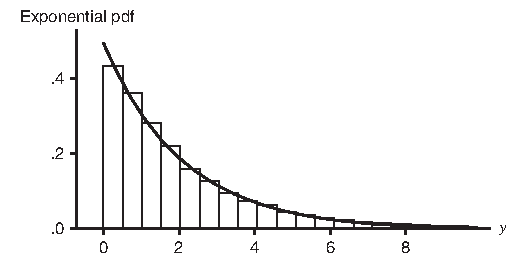
\includegraphics[width=.60\textwidth]{assets/chapter5/fig-5-6-1.pdf}
\caption{从$\lambda=2$的指数pdf生成的10,000个观测的直方图及其pdf}\label{fig:5.6.1}
\end{figure}\par
指数分布与其他分布的关系，使许多随机变量可以快速生成.例如，若$U_i$为iid $\operatorname{uniform}(0,1)$随机变量，则
\begin{equation}\label{eq:5.6.5}\index{SI0255@生成}\index{SI0281@生成}\index{SI0307@生成}\index{SI0361@生成}
\begin{aligned}
Y&=-2\sum_{j=1}^\nu\log(U_j)\sim\chi_{2\nu}^2,\\
Y&=-\beta\sum_{j=1}^a\log(U_j)\sim\operatorname{gamma}(a,\beta),\\
Y&=\frac{\sum_{j=1}^a\log(U_j)}{\sum_{j=1}^{a+b}\log(U_j)}\sim\operatorname{beta}(a,b).
\end{aligned}
\end{equation}
还可以作许多变形（见\autoref{exercise:5.47}—\autoref{exercise:5.49}），但都由指数—均匀变换导出.

遗憾的是，这一变换有局限.例如，不能用它生成奇数自由度的$\chi^2$随机变量，所以不能得到$\chi_1^2$，进而得到极其有用的$\operatorname{normal}(0,1)$随机变量.下一小节会再讨论此问题.

回顾\autoref{ex:5.6.3}以及\eqref{eq:5.6.5}中各变换的基础，都是概率积分变换，一般可写成
\begin{equation}\label{eq:5.6.6}
F_Y^{-1}(u)=y\iff u=\int_{-\infty}^y f_Y(t)\,dt.
\end{equation}
将此公式用于指数分布尤其方便，因为积分方程有简单解（另见\autoref{exercise:5.59}）.但很多情况下\eqref{eq:5.6.6}没有闭式解，于是每生成一个随机变量都要解一次积分方程，实践中可能过于耗时和复杂.例如，用\eqref{eq:5.6.6}生成$\chi_1^2$就有这个问题.

没有闭式解时，应探索其他办法，包括其他类型的生成方法以及间接方法.下面是前一类方法的例子.
\begin{example}[{\hyperref[bib:source46]{Box–Muller，1958}}]\label{ex:5.6.4}\index{SI0099@Box–Muller变换}\index{SI1038@Box–Muller}
生成两个独立的$\operatorname{uniform}(0,1)$随机变量$U_1$和$U_2$，令
$$R=\sqrt{-2\log U_1},\qquad\theta=2\pi U_2.$$
则
$$X=R\cos\theta,\qquad Y=R\sin\theta$$
\sourcepageanchor{234}
是独立的$\operatorname{normal}(0,1)$随机变量.所以，虽然没有生成单个$n(0,1)$变量的快速变换，却有一次生成两个变量的方法（见\autoref{exercise:5.50}）.
\end{example}
遗憾的是，\autoref{ex:5.6.4}这样的解法并不多.它们还利用了特定分布的结构，因此不太适合作为一般策略.对于其他尚未讨论的连续分布，多数时候最好用间接方法生成.在探索这些方法之前，先以离散随机变量的情形结束本小节；此时\eqref{eq:5.6.6}很有用.

若离散随机变量$Y$的取值为$y_1<y_2<\cdots<y_k$，类似\eqref{eq:5.6.6}可写
\begin{equation}\label{eq:5.6.7}
\begin{aligned}
P[F_Y(y_i)\le U<F_Y(y_{i+1})]&=F_Y(y_{i+1})-F_Y(y_i)\\
&=P(Y=y_{i+1}).
\end{aligned}
\end{equation}
实际用\eqref{eq:5.6.7}生成离散随机变量很直接，可概括如下.为生成$Y_i\sim F_Y(y)$：
\begin{enumerate}[label=\textbf{\alph*.}]
\item 生成$U\sim\operatorname{uniform}(0,1)$.
\item 若$F_Y(y_i)\le U<F_Y(y_{i+1})$，令$Y=y_{i+1}$.
\end{enumerate}
定义$y_0=-\infty$及$F_Y(y_0)=0$.
\begin{example}[二项随机变量的生成]\label{ex:5.6.5}\index{SI0263@生成}\index{SI0286@生成}
例如，为生成$Y\sim\operatorname{binomial}(4,5/8)$，生成$U\sim\operatorname{uniform}(0,1)$并令
\begin{equation}\label{eq:5.6.8}
Y=\begin{cases}0,&0\le U<.020,\\1,&.020\le U<.152,\\2,&.152\le U<.481,\\3,&.481\le U<.847,\\4,&.847\le U\le1.\end{cases}
\end{equation}
\end{example}
即使离散随机变量的值域无限，如Poisson或负二项分布，\eqref{eq:5.6.8}中的算法也适用.理论上这可能需要大量求值，但实际上有简单巧妙的加速方法，因而通常不会如此.例如，不必按$1,2,\ldots$的次序逐个检查$y_i$，从靠近均值的$y_i$开始可能快得多（见\hyperref[bib:source253]{Ripley 1987}，第3.3节，以及\autoref{exercise:5.55}）.

后面将看到模拟方法的许多用途.先考察下面对Poisson分布的探索，它是\autoref{sec:10.1.4}将介绍的参数自助法（parametric bootstrap）的一个版本.
\begin{example}[Poisson方差的分布]\label{ex:5.6.6}\index{SI0096@参数}\index{SI0752@参数自助法}
若$X_1,\ldots,X_n$为iid $\operatorname{Poisson}(\lambda)$，由\autoref{thm:5.2.7}或\autoref{thm:5.2.11}，$\sum X_i$服从$\operatorname{Poisson}(n\lambda)$.因此很容易描述样本均值$\bar X$的分布，但描述样本方差$S^2=\frac1{n-1}\sum(X_i-\bar X)^2$的分布并不容易.

不过，$S^2$的分布很容易模拟.例如，取$n=5$，从$\operatorname{Poisson}(\lambda)$分布生成1,000个容量为5的样本.\autoref{fig:5.6.2}给出这些样本的直方图.\footnote{译注：此处原文的1,000个、容量5的设定，与图及后文实际使用的5,000个、容量13的设定不一致.图题和后续计算均按原文保留.}此外，模拟样本还能计算关于$S^2$的概率.若$S_i^2$为第$i$个模拟样本计算出的值，则
$$\frac1M\sum_{i=1}^M I(S_i^2\ge a)\to P_\lambda(S^2\ge a),\qquad M\to\infty.$$
\sourcepageanchor{235}
\par\begin{figure}[H]\centering
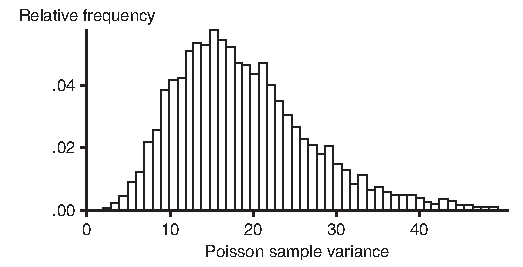
\includegraphics[width=.60\textwidth]{assets/chapter5/fig-5-6-2.pdf}
\caption{从$\lambda=18.69$的Poisson分布抽取5,000个容量为13的样本所得样本方差$S^2$的直方图.这5,000个数值的均值与标准差为18.86和7.68}\label{fig:5.6.2}
\end{figure}\par
为说明这种方法的用途，考虑1984年8月下旬在哈德逊河取得的海湾{\upshape\CJKfontspec{SimSun}鳀}鱼幼体计数样本：
\begin{equation}\label{eq:5.6.9}
19,32,29,13,8,12,16,20,14,17,22,18,23.
\end{equation}
若假定幼体在河中随机且均匀分布，则固定大小渔网捕获的数量应服从Poisson分布.这一论证来自Poisson公设的空间版本（见\autoref{sec:2.6}）.为考察假设是否合理，可检查观测数据的均值和方差是否符合Poisson假设.

对\eqref{eq:5.6.9}的数据，计算得$\bar x=18.69$、$s^2=44.90$.Poisson假设下，预期两者相同.当然，由于抽样变异，它们不会完全相同，可用模拟了解应有的差异.\autoref{fig:5.6.2}中，从$\lambda=18.69$的Poisson分布模拟5,000个容量为$n=13$的样本，构造$S^2$的相对频数直方图.观测值$S^2=44.90$落在分布尾部.事实上，有27个$S^2$值大于44.90，故可估计
$$P(S^2>44.90\mid\lambda=18.69)=\frac1{5000}\sum_{i=1}^{5000}I(S_i^2>44.90)=\frac{27}{5000}=.0054,$$
这使我们怀疑Poisson假设；见\autoref{exercise:5.54}.（这类发现催生了一个很糟糕的双语双关：“哈德逊河里有些‘鱼’常——Poisson失效了.”\footnote{译注：原文为“Something is fishy in the Hudson—the Poisson has failed.”英语fishy兼有“鱼腥的”与“可疑的”之意；Poisson与法语“鱼”poisson同形.}）
\end{example}
\subsubsection{间接方法}\label{sec:5.6.2}
找不到容易的直接变换来生成所需随机变量时，一种非常有力的间接方法——接受／拒绝算法（Accept/Reject Algorithm）——常能提供解法.它的思想或许最好用一个简单例子说明.
\begin{example}[beta随机变量的生成——I]\label{ex:5.6.7}\index{SI0001@接受／拒绝算法}\index{SI0006@接受／拒绝}\index{SI0255@生成}
设目标是生成$Y\sim\operatorname{beta}(a,b)$.若$a,b$都是整数，可用直接变换法\eqref{eq:5.6.5}；若不是整数，该方法就不适用.具体取$a=2.7$、$b=6.3$.\autoref{fig:5.6.3}把beta密度$f_Y(y)$放在边长为1和$c\ge\max_yf_Y(y)$的长方形里.考虑以下计算$P(Y\le y)$的方法.若$(U,V)$为独立的$\operatorname{uniform}(0,1)$随机变量，则阴影区域的概率为
\sourcepageanchor{236}
\begin{equation}\label{eq:5.6.10}
\begin{aligned}
P\left(V\le y,U\le\frac1c f_Y(V)\right)&=\int_0^y\int_0^{f_Y(v)/c}\,du\,dv\\
&=\frac1c\int_0^y f_Y(v)\,dv\\
&=\frac1cP(Y\le y).
\end{aligned}
\end{equation}
\par\begin{figure}[H]\centering
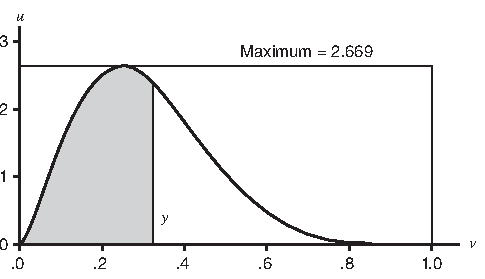
\includegraphics[width=.62\textwidth]{assets/chapter5/fig-5-6-3.pdf}
\caption{$a=2.7$、$b=6.3$的beta分布，$c=\max_yf_Y(y)=2.669$.均匀随机变量$V$给出横坐标，利用$U$判断是否处于密度曲线下方}\label{fig:5.6.3}
\end{figure}\par
所以可以从均匀分布的概率算出beta概率，这提示可从均匀随机变量生成beta随机变量.

在\eqref{eq:5.6.10}中令$y=1$，得$1/c=P(U<(1/c)f_Y(V))$，因此
\begin{equation}\label{eq:5.6.11}
\begin{aligned}
P(Y\le y)&=\frac{P(V\le y,U\le(1/c)f_Y(V))}{P(U\le(1/c)f_Y(V))}\\
&=P(V\le y\mid U\le(1/c)f_Y(V)),
\end{aligned}
\end{equation}
这提示如下算法.为生成$Y\sim\operatorname{beta}(a,b)$：
\begin{enumerate}[label=\textbf{\alph*.}]
\item\label{item:5.6.7a} 生成独立的$\operatorname{uniform}(0,1)$变量$(U,V)$.
\item\phantomsection\label{itm:ex:5.6.7:b} 若$U<(1/c)f_Y(V)$，令$Y=V$；否则返回步骤\hyperref[item:5.6.7a]{a}.
\end{enumerate}
只要$c\ge\max_yf_Y(y)$，这一算法就能生成$\operatorname{beta}(a,b)$随机变量；实际上还可推广到支撑集有界的任意密度（\autoref{exercise:5.59}和\autoref{exercise:5.60}）.
\end{example}
显然，$c$的最佳选择是$c=\max_yf_Y(y)$.为说明理由，注意该算法的运行次数不固定：不知道要获得一个$Y$需要多少对$(U,V)$.但若定义随机变量
\begin{equation}\label{eq:5.6.12}
N=\text{生成一个$Y$所需的$(U,V)$对数},
\end{equation}
回顾$1/c=P(U\le(1/c)f_Y(V))$，有
$$\begin{aligned}P(N=1)&=\frac1c,\\P(N=2)&=\left(1-\frac1c\right)\frac1c,\\&\ \vdots\end{aligned}$$
\sourcepageanchor{237}
所以$N$是几何随机变量.因此，为生成一个$Y$，平均需要$E(N)=c$对$(U,V)$；从这一意义上，最小化$c$会使算法最优.

由\autoref{fig:5.6.3}可见，$U>(1/c)f_Y(V)$区域造成浪费，这是因为用均匀随机变量$V$生成beta随机变量$Y$.为改进，可以从更接近beta的分布开始.

算法的检验步骤\hyperref[itm:ex:5.6.7:b]{(b)}可理解为检查随机变量$V$是否“看起来像”来自密度$f_Y$.设$V\sim f_V$，计算
$$M=\sup_y\frac{f_Y(y)}{f_V(y)}<\infty.$$
步骤\hyperref[itm:ex:5.6.7:b]{(b)}的一般化，是比较$U\sim\operatorname{uniform}(0,1)$与$(1/M)f_Y(V)/f_V(V)$.比值越大，$V$越“像”来自随机密度$f_Y$，越有可能满足$U<(1/M)f_Y(V)/f_V(V)$.这就是一般接受／拒绝算法的基础.
\subsubsection{接受／拒绝算法}\label{sec:5.6.3}
\begin{theorem}\label{thm:5.6.8}\index{SI0001@接受／拒绝算法}\index{SI0006@接受／拒绝}
设$Y\sim f_Y(y)$、$V\sim f_V(V)$，其中$f_Y$和$f_V$有共同支撑集，且
$$M=\sup_y f_Y(y)/f_V(y)<\infty.$$
为生成随机变量$Y\sim f_Y$：
\begin{enumerate}[label=\textbf{\alph*.}]
\item\label{item:5.6.8a} 生成独立的$U\sim\operatorname{uniform}(0,1)$和$V\sim f_V$.
\item 若$U<(1/M)f_Y(V)/f_V(V)$，令$Y=V$；否则返回\hyperref[item:5.6.8a]{第一步}.
\end{enumerate}
\end{theorem}
\begin{proof}
生成的随机变量$Y$具有cdf
\begin{align*}
P(Y\le y)&=P(V\le y\mid\text{停止})\\
&=P(V\le y\mid U<(1/M)f_Y(V)/f_V(V))\\
&=\frac{P(V\le y,U<(1/M)f_Y(V)/f_V(V))}{P(U<(1/M)f_Y(V)/f_V(V))}\\
&=\frac{\displaystyle\int_{-\infty}^y\int_0^{(1/M)f_Y(v)/f_V(v)}\,du\,f_V(v)\,dv}{\displaystyle\int_{-\infty}^\infty\int_0^{(1/M)f_Y(v)/f_V(v)}\,du\,f_V(v)\,dv}\\
&=\int_{-\infty}^y f_Y(v)\,dv,
\end{align*}
正是所需cdf.
\end{proof}
另注意
$$\begin{aligned}
M&=\sup_yf_Y(y)/f_V(y)\\
&=[P(U<(1/M)f_Y(V)/f_V(V))]^{-1}\\
&=\frac1{P(\text{停止})},
\end{aligned}$$
所以生成一个$Y$所需的试验次数服从$\operatorname{geometric}(1/M)$，$M$为期望试验次数.
\sourcepageanchor{238}
\begin{example}[beta随机变量的生成——II]\label{ex:5.6.9}\index{SI0255@生成}
为生成$Y\sim\operatorname{beta}(2.7,6.3)$，考虑算法：
\begin{enumerate}[label=\textbf{\alph*.}]
\item\label{item:5.6.9a} 生成$U\sim\operatorname{uniform}(0,1)$、$V\sim\operatorname{beta}(2,6)$.
\item 若$U<(1/M)f_Y(V)/f_V(V)$，令$Y=V$；否则返回\hyperref[item:5.6.9a]{第一步}.
\end{enumerate}
只要$\sup_y f_Y(y)/f_V(y)\le M<\infty$，该接受／拒绝算法就生成所需的$Y$.对给定密度有$M=1.67$，满足要求（见\autoref{exercise:5.63}）.

这一算法有$EN=1.67$，而\autoref{ex:5.6.7}中使用均匀$V$的算法有$EN=2.67$.虽然这似乎说明后一算法更快，\footnote{译注：原文此处为“latter algorithm”，但按前面的试验次数比较，应指当前使用beta候选的前一算法.随后关于每次生成成本的提醒仍然成立.}别忘了生成一个$\operatorname{beta}(2,6)$变量需要八个均匀随机变量.所以比较算法不总是直接的，还须同时考虑计算机速度和编程便利性.
\end{example}
必须强调$M<\infty$的重要性.它可理解为要求$V$的密度（常称候选密度，candidate density）的尾部比$Y$的密度（常称目标密度，target density）更重.这有助于保证$Y$的各种值、包括尾部值，都得到良好代表.例如，若$V\sim\operatorname{Cauchy}$、$Y\sim n(0,1)$，预期$V$样本的范围宽于$Y$样本，因此基于这两个密度的接受／拒绝算法应有良好表现.反过来，把$n(0,1)$变量变成Cauchy变量就困难得多，因为极端值的代表不足.

但有时目标密度具有重尾，难以找到使$M$有限的候选密度.此时接受／拒绝算法不再适用，便引出另一类方法，称为马尔可夫链Monte Carlo方法（Markov Chain Monte Carlo，MCMC）.其特例包括Gibbs抽样器（Gibbs Sampler）和Metropolis算法.下面给出后者.

\noindent\textbf{Metropolis算法.}\index{SI0015@Metropolis}\semanticindexanchor{15:238}\index{SI0688@Metropolis算法}\semanticindexanchor{688:238} 设$Y\sim f_Y(y)$、$V\sim f_V(v)$，其中$f_Y$和$f_V$有共同支撑集.为生成$Y\sim f_Y$：
\begin{enumerate}[label=\arabic*.,start=0]
\item 生成$V\sim f_V$，令$Z_0=V$.
\end{enumerate}
对$i=1,2,\ldots$：
\begin{enumerate}[label=\arabic*.]
\item 生成$U_i\sim\operatorname{uniform}(0,1)$、$V_i\sim f_V$，计算
$$\rho_i=\min\left\{\frac{f_Y(V_i)}{f_V(V_i)}\cdot\frac{f_V(Z_{i-1})}{f_Y(Z_{i-1})},1\right\}.$$
\item 令
$$Z_i=\begin{cases}V_i,&U_i\le\rho_i,\\Z_{i-1},&U_i>\rho_i.\end{cases}$$
\end{enumerate}
则当$i\to\infty$时，$Z_i$依分布收敛到$Y$.

虽然算法不要求$M$有限，但它并不生成密度恰为$f_Y$的随机变量，而是产生一个收敛序列.实际运行一段时间后（$i$变大），产生的$Z$的表现就很接近来自$f_Y$的变量.（关于Metropolis算法的初步介绍，见Chib和Greenberg.）
\sourcepageanchor{239}
虽然MCMC方法至少可追溯到\hyperref[bib:source219]{Metropolis等（1953）}，但它们真正受到广泛重视，是在\hyperref[bib:source137]{Geman和Geman（1984）}的基础上，随着\hyperref[bib:source134]{Gelfand和Smith（1990）}的工作而发生的.更多内容见\autoref{sec:5.8.5}.
